\subsection{\textsc{AvaDam}} \label{sec:designAvaDam}
%Jens
%Er der instruktioner i hvordan spillet spilles?
\textbf{Brugervejledning:} \textsc{AvaDam} har ingen direkte brugervejledning i hvordan dam spillet spilles. Det antages at brugeren er kendt med dam, og specifikt danskdam.dk's regelsæt\footnote{Dansk Dam Forenings officielle hjemmeside: \url{http://www.danskdam.dk/}}, da det er dette spillet håndhæver. I alle tilfælde er spillets gang præsenteret på en intuitiv måde (fx via visuelle vink) så en uvidendende bruger højst sandsynligt hurtigt lærer de basale regler af spillet, blot ved at spille. \\

%Jens
%Hvilke regelsæt benyttes?
\textbf{Regelsæt:} \textsc{AvaDam}s regler tager udgangspunkt i det regelsæt der er redegjort af Dansk Dam Forening. Den eneste undtagelse af dette er hvorvidt en combo \textit{skal} fuldføres eller kan stoppes undervejs. Her er Dansk Dam Forenings regelbeskrivelse tvetydige og reglen er derfor blevet indført som en valgfri mulighed i spilindstillingerne.  \\

% Magnus
% Hvordan ved spilleren inde i spillet, hvilke regler der er på?
\textbf{Aktiverede regler:} Der er mange mulige regler i dam. De grundlæggende regler er altid aktive; Hvert felt kan kun have én brik stående. Brikker kan kun flytte diagonalt. Spilleren kan ikke slå sine egne brikker ihjel. \textsc{AvaDam} har dog yderligere regler, der kan aktiveres gennem menuen i checkbokse. De kan genkendes inde i spillet gennem visuelle vink. De aktivérbare regler er kort:

\begin{figure}[H]
    \centering
    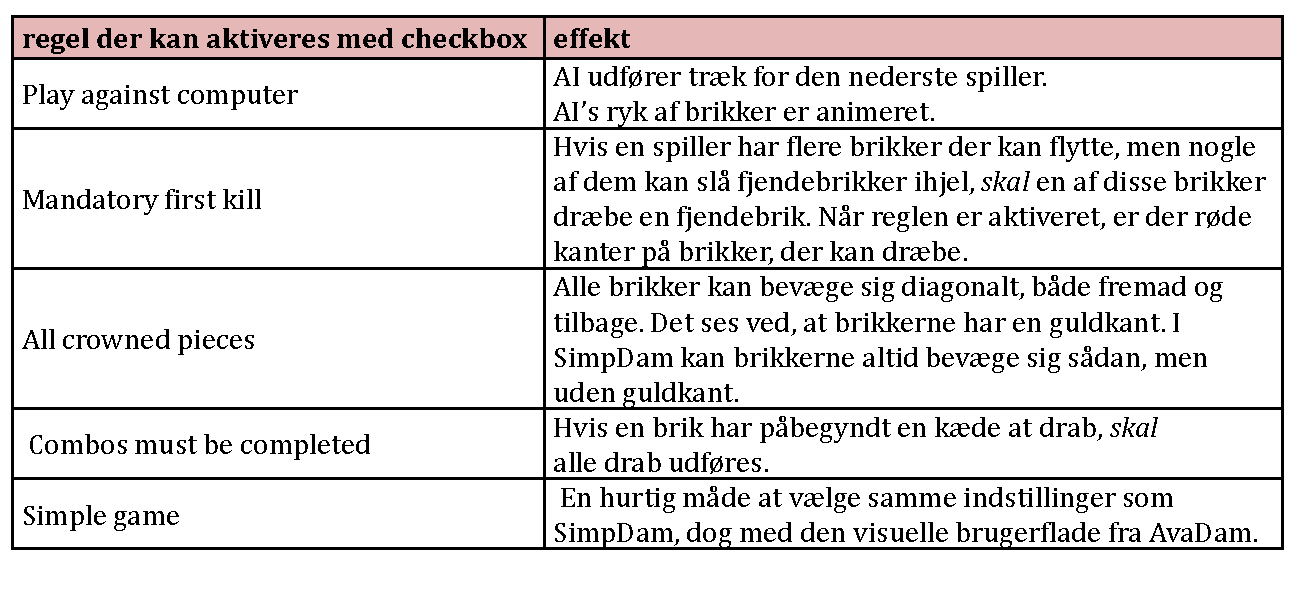
\includegraphics[width = 1.0 \textwidth]{Figurer/aktiveredeRegler.pdf}
    \caption{Aktivérbare regler i det \textsc{AvaDam}, og deres tilhørende effekt på spillet.}
    \label{fig:aktiveredeRegler}
\end{figure}

% Magnus
% Hvad betyder pointene?

\textbf{Score:} I \textsc{AvaDam} får hver spiller point for at flytte en brik (+1 point), og yderligere 9 point for at slå en fjendebrik ihjel. Pointene lagres i modellen \texttt{DamModel} i static fields. Scorene vises i panelet til højre for brættet.\\

%Jens 
%Nedenstående fire spørgsmål er placeret under samme kategori: visuelle indikatorer
%\item Hvordan ved jeg, hvilke legale træk en brik har?
%\item Hvad er forskellen på grøn og gult highlight?
%\item Hvad betyder kantfarverne? rød + gul.
%\item Hvordan genkender jeg en kronet brik?

\textbf{Visuelle indikatorer:} For at holde brugeren opdateret på spillets gang og for at håndhæve spillets regler, er der designet tre typer visuelle indikatorer; farvede kanter på brikker, farve fremhævning af felter og gennemsigtighed af brikker. 
\begin{enumerate}
    \item For at klargøre hvilken spillers tur det er bliver den ikke-aktive spillers brikker gjort 30\% mere gennemsigtige.
    
    \item For at vise særligt gældende regler/egenskaber for bestemte brikker, farveslægges disse brikkers kanter. En kronet brik, får en gyldengul kant når de bliver kronet. Hvis indstillingen \texttt{"Mandatory first kill"} er valgt, får aktive-spillers brikker, som kan udføre et drab, ændret kantfarve til rød. Hvis en brik har rød kant, er det den eneste brik der kan rykkes. Hvis flere brikker har rød kant vælges frit mellem disse. Indikationerne ses bl.a. på forsidens figur. 
    
    \item For at vise hvilke legale træk der kan tages med en valgt brik, bliver samtlige mulige legale felter fremhævet med én af to farver. Felter fremhævet med lysegrøn repræsenterer mulige felter hvor trækket kan afsluttes, se figur \ref{fig:MovePieceFigure}. \begin{figure}[H]
        \centering
        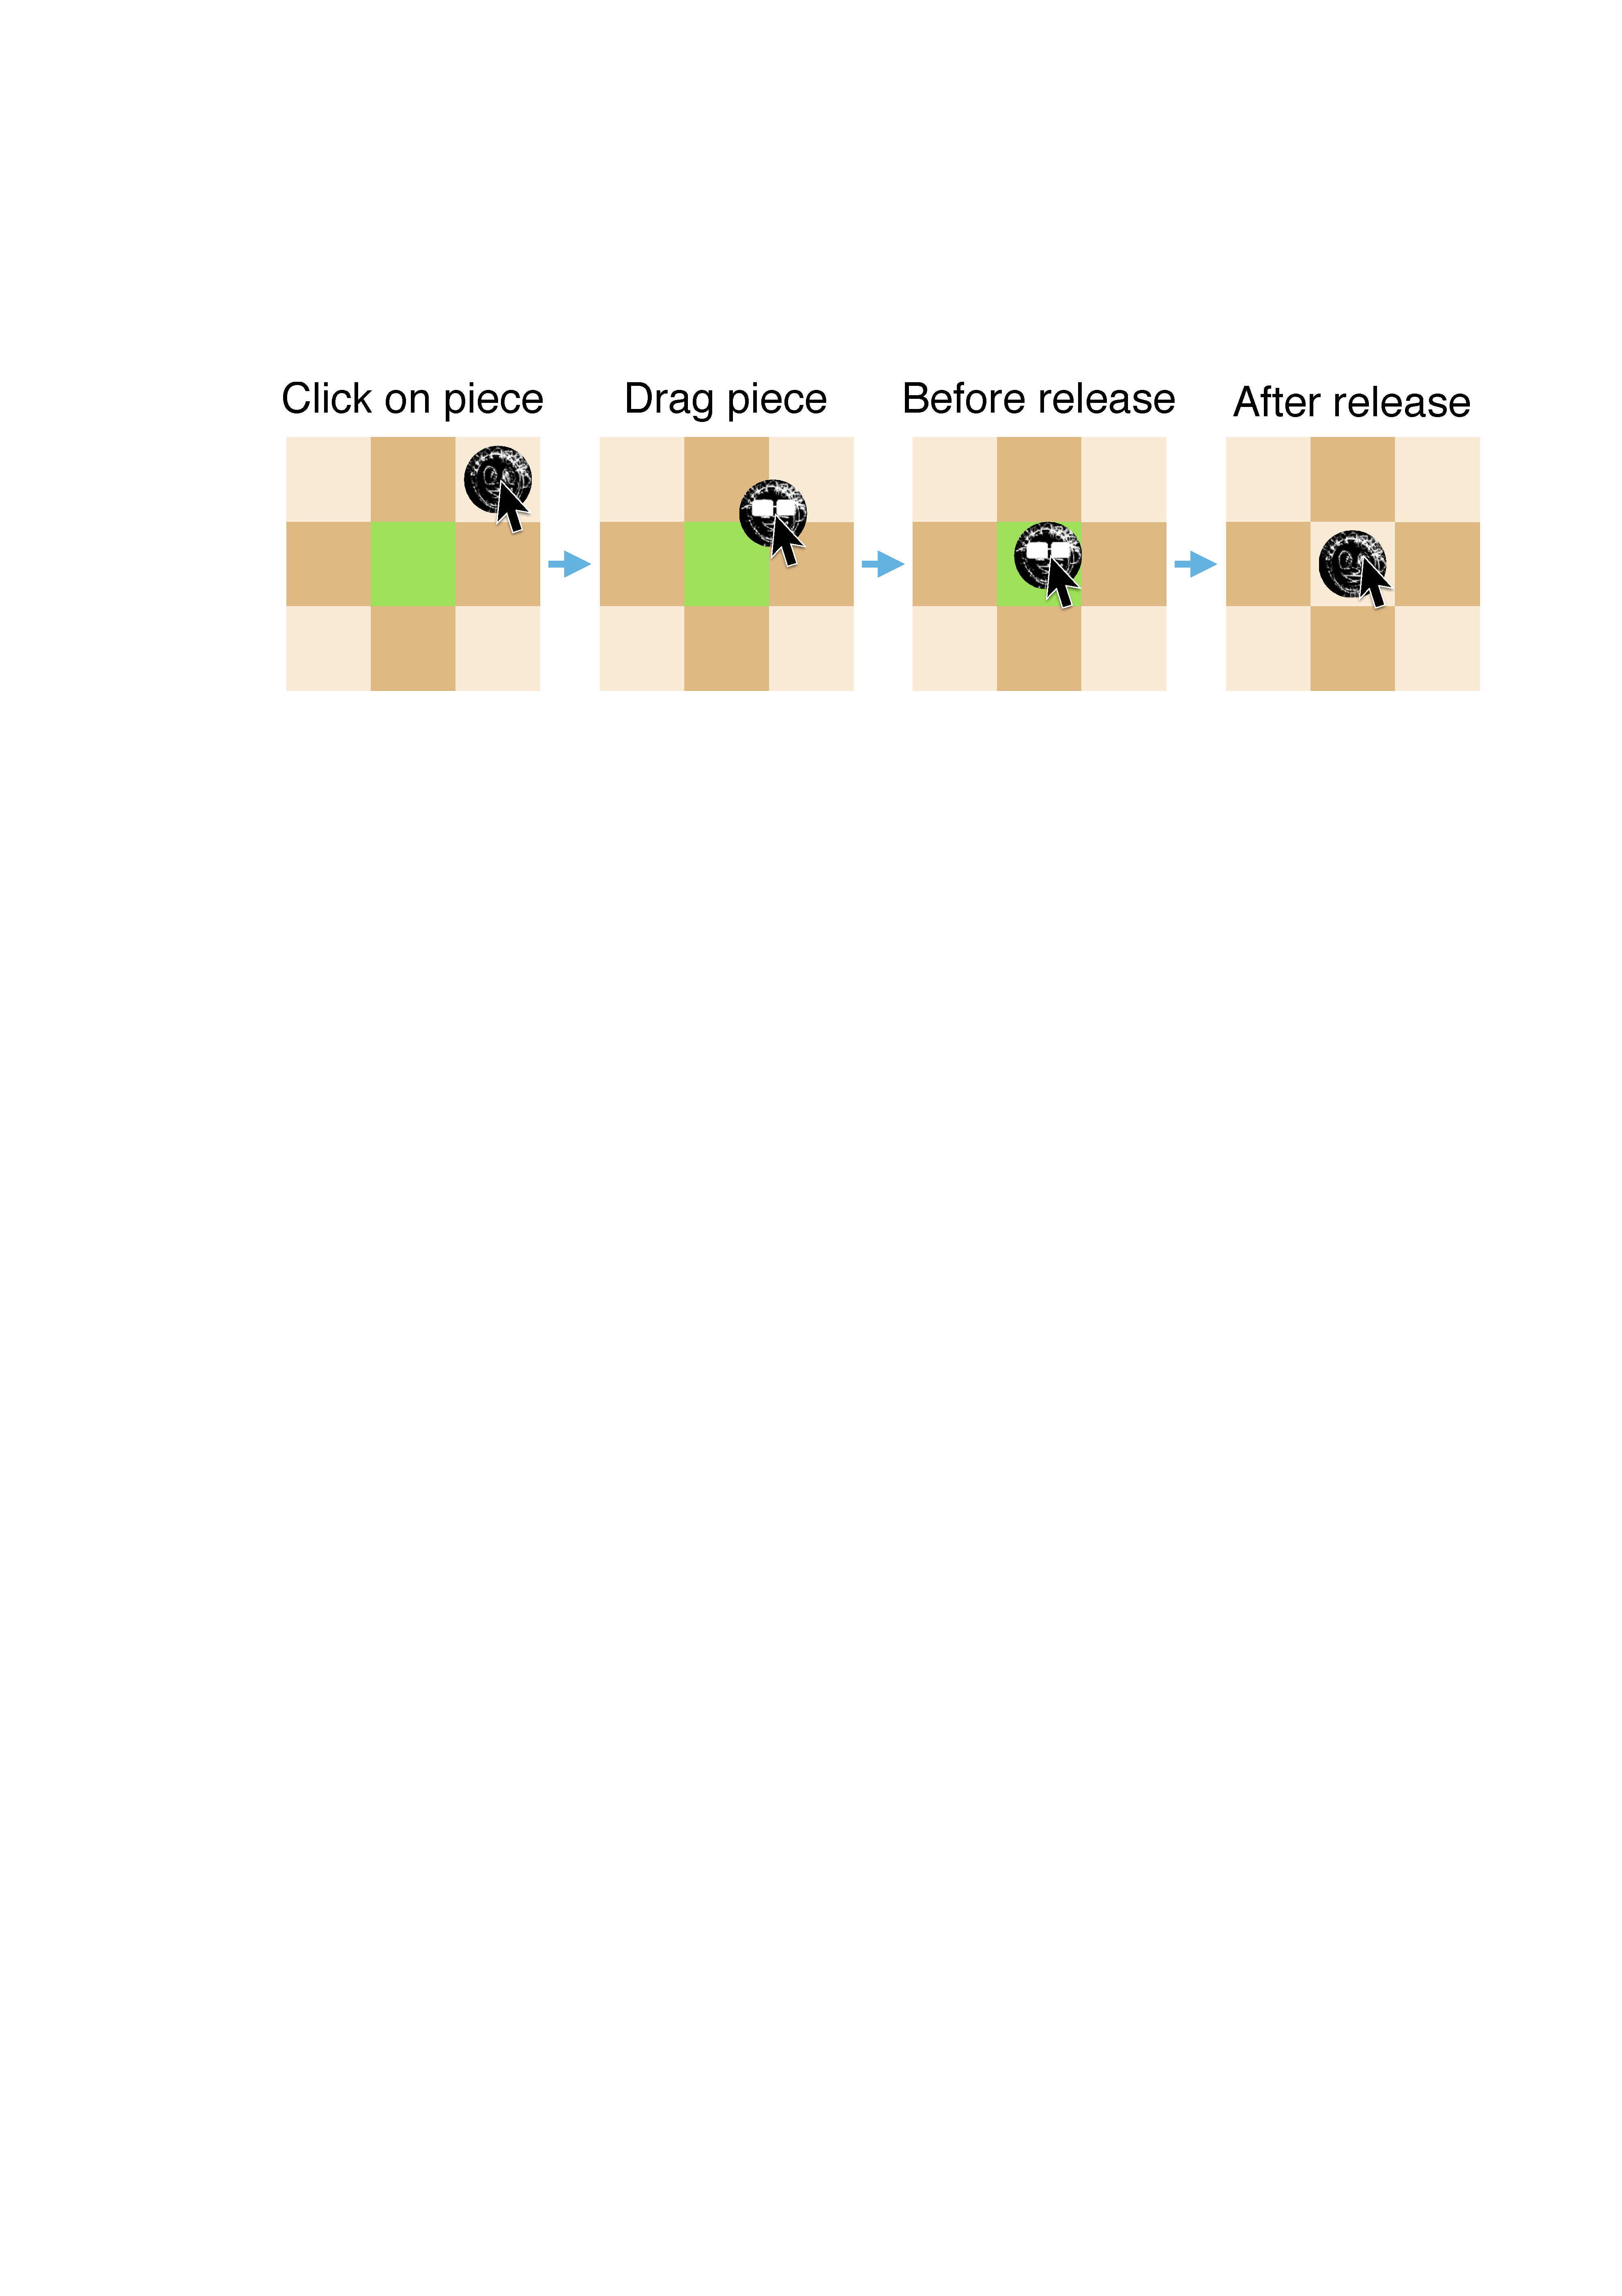
\includegraphics[width = \textwidth]{Figurer/MovePieceFigure}
        \caption{Illustration over hvordan legale felter fremhæves med lysegrøn farve når en brik vælges.}
        \label{fig:MovePieceFigure}
    \end{figure}

    Hvis trækket involvere et drab, vil et grønt felt skifte farve til gyldengul, når den markeres over. Dette indikere at en combo er påbegyndt. Hvis det ud fra det nyligt markeret gule felt er muligt at lave endnu et drab med samme brik, vil dette korresponderende felt nu lyse op med grønt - og således foreslå et nyt legalt afslutningsfelt. Spilleren kan nu vælge at fortsætte sin combo eller at afslutte den på det gule felt ved at slippe musemarkøren\footnote{I spilindstillingerne kan færdiggørelsen af en combo gøres obligatorisk}. Spilleren fortætter comboen ved at markere det nye grønne felt og dermed gøre det gult. Til slut, før musemarkøren slippes, viser de gule felter den rute som brikken "bevæger" sig over i løbet af trækket. Se nedenstående figur \ref{fig:ComboFigure}.
     \begin{figure}[H]
        \centering
        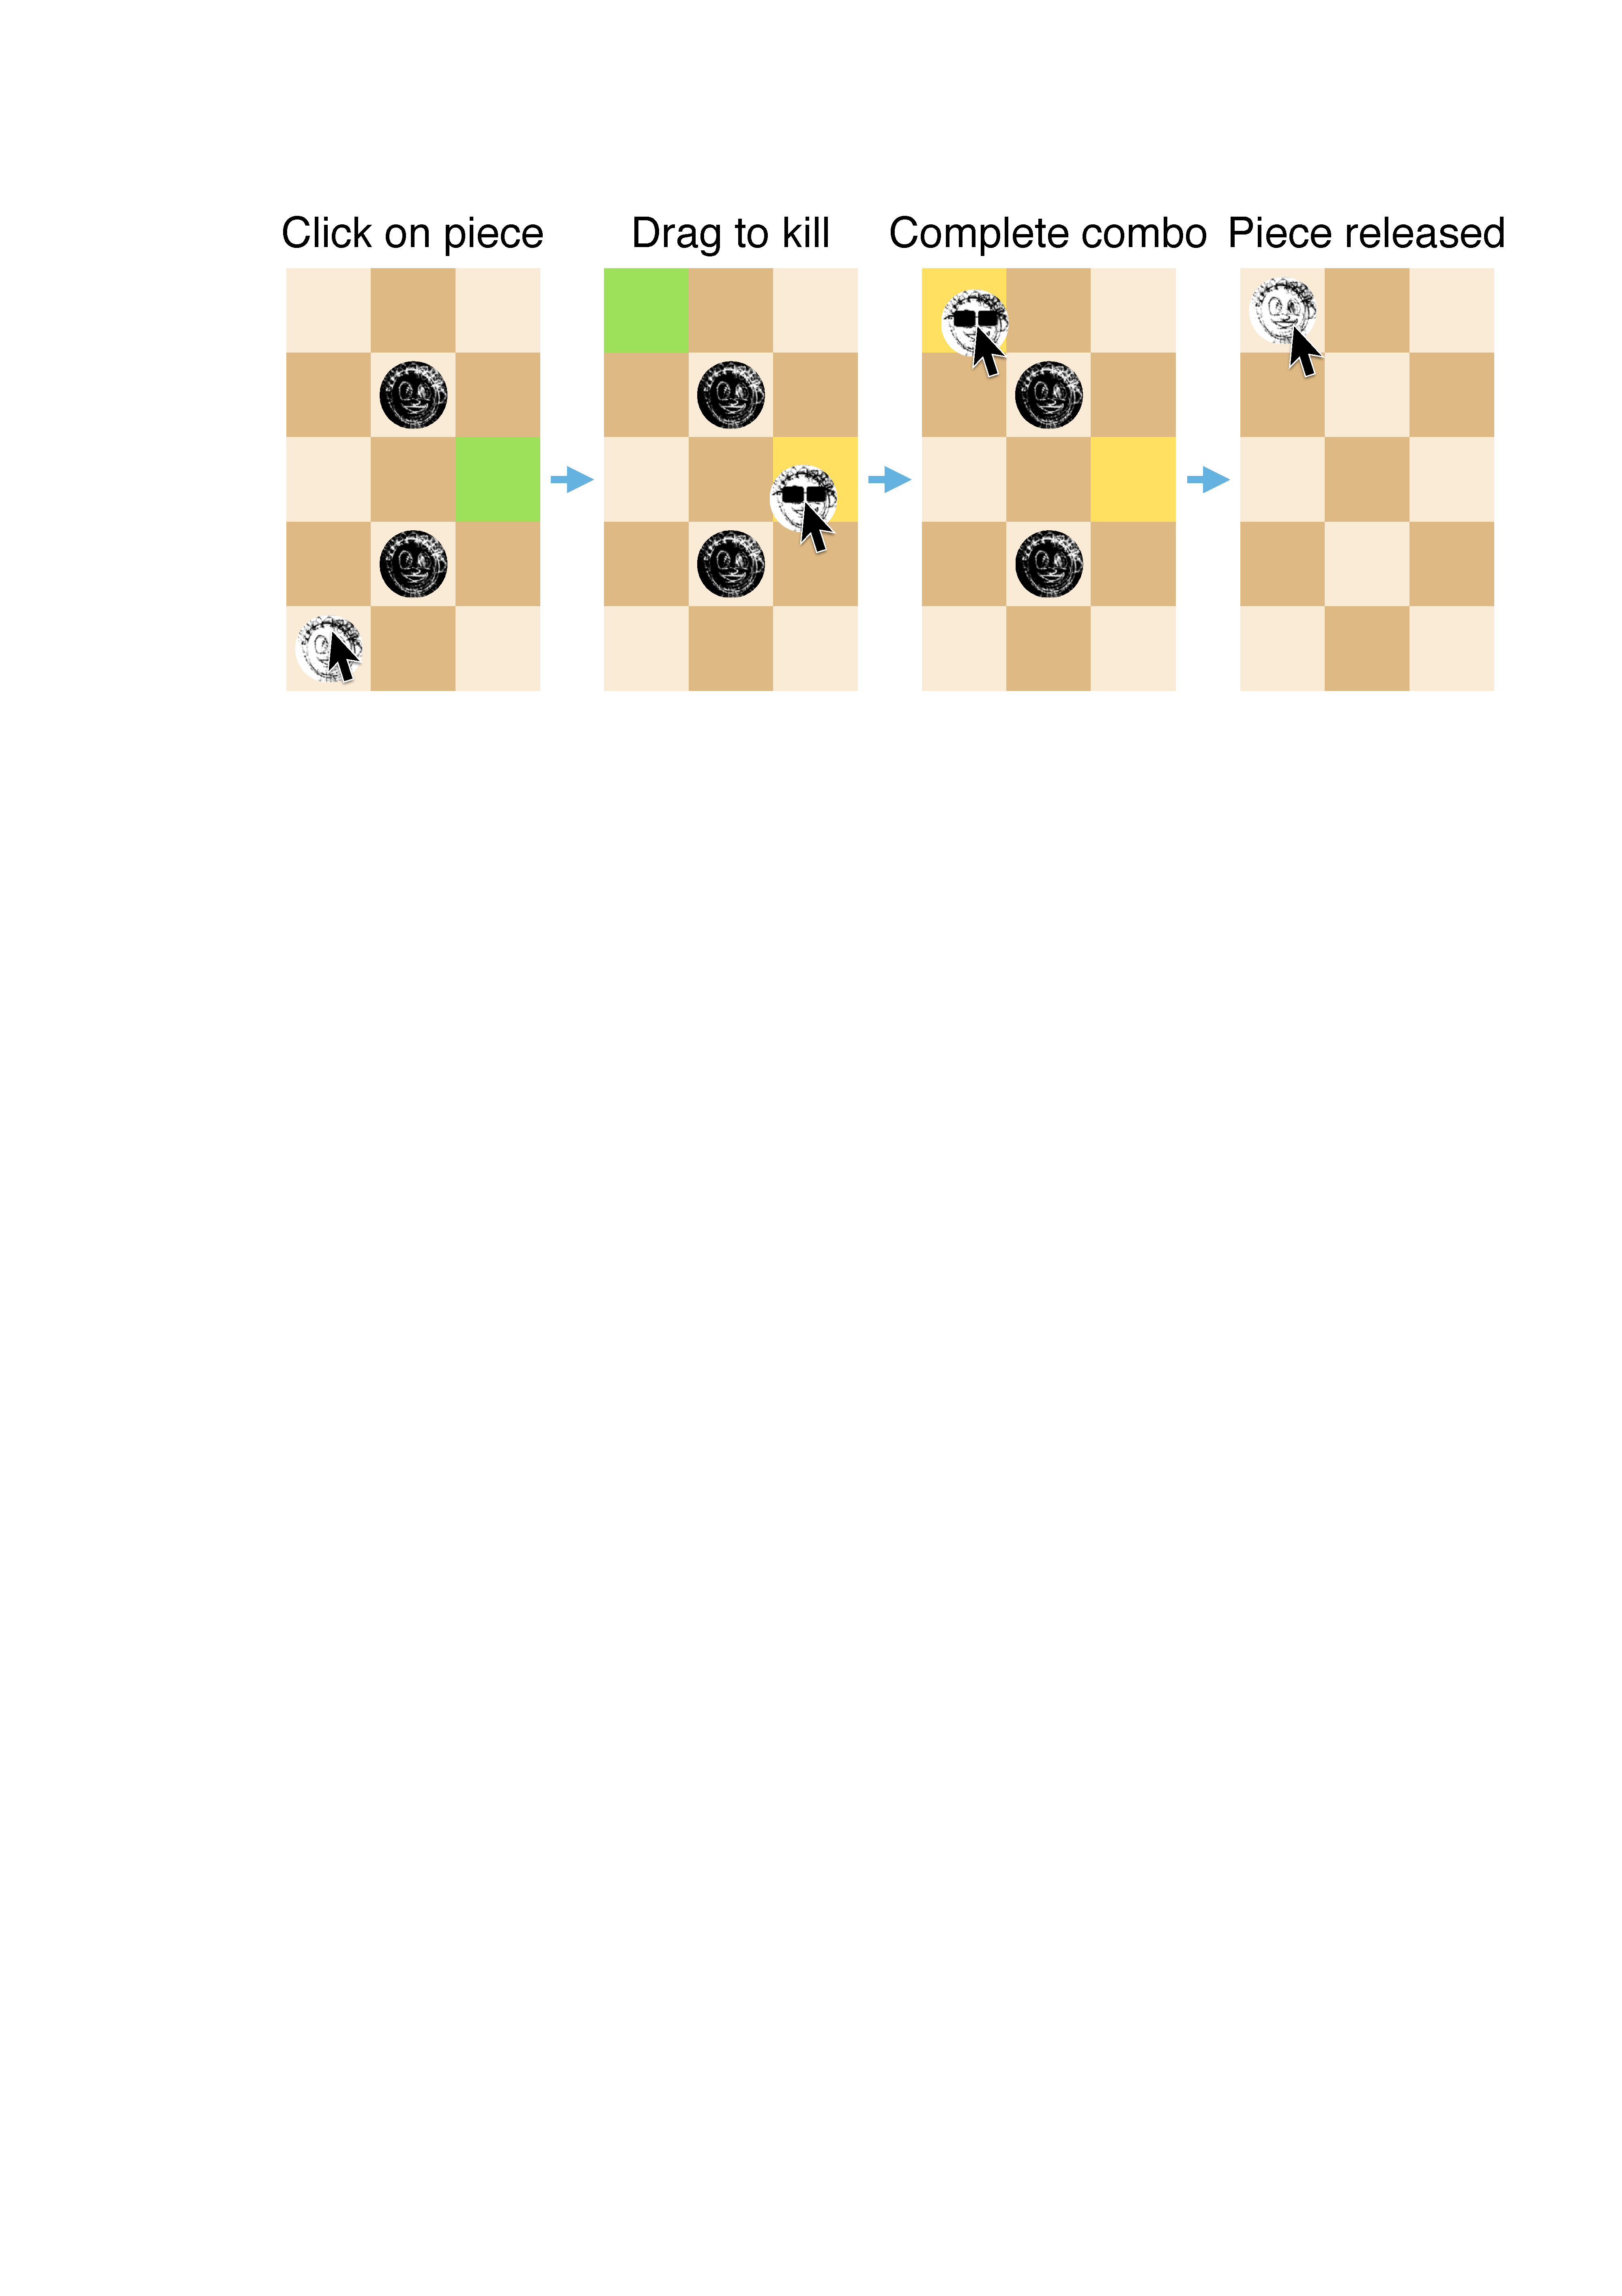
\includegraphics[width = \textwidth]{Figurer/ComboFigure}
        \caption{Figur over hvordan udførelsen af en combo bliver indikeret og udført.}
        \label{fig:ComboFigure}
    \end{figure}
\end{enumerate}
  
%Jens
%Hvordan ændrer jeg brætstørrelse? (slider)
\textbf{Brætstørrelse:} Inde i spilindstillingerne findes en slider som kan justere størrelsen af brættet. Denne effekt træder først i kraft når en nyt spil startes.\\

% Magnus
% Hvordan skalerer spillet på større/mindre skærme? (begge)
% Er resizing muligt undervejs? (advdam)
\textbf{Skalering på skærme og resizing:} Da størrelsen af vores tegnede shapes er baseret på view koordinater, der skaleres efter scenens størrelse, skaleres spilvinduet efter programbrugerens skærmstørrelse (eller egt. opløsning). Til forskel fra \textsc{SimpDam}, er der i \textsc{AvaDam} forskel på scenens vidde og højde; panelet med score og uafgjort knapper til højre er dog også skaleret efter skærmens højde. Det er ikke muligt at ændre vinduets størrelse ved at trække i vinduets hjørne. \\

%   RR
%   \item Hvad er gjort for at gøre spillet underholdende? (advdam)
\textbf{Underholdning i spillet:} 
For at bringe yderligere underholdning ind i spillet er der tilføjet at brugeren kan skifte billeder (samt gifs) for hvert holds brikker. Eksempler på disse billeder ses i figur \ref{fig:ShowcasePieces}. Vi har også introduceret forskellige spilleregler for at indføre variation.
\\
\begin{figure}[H]
    \centering
    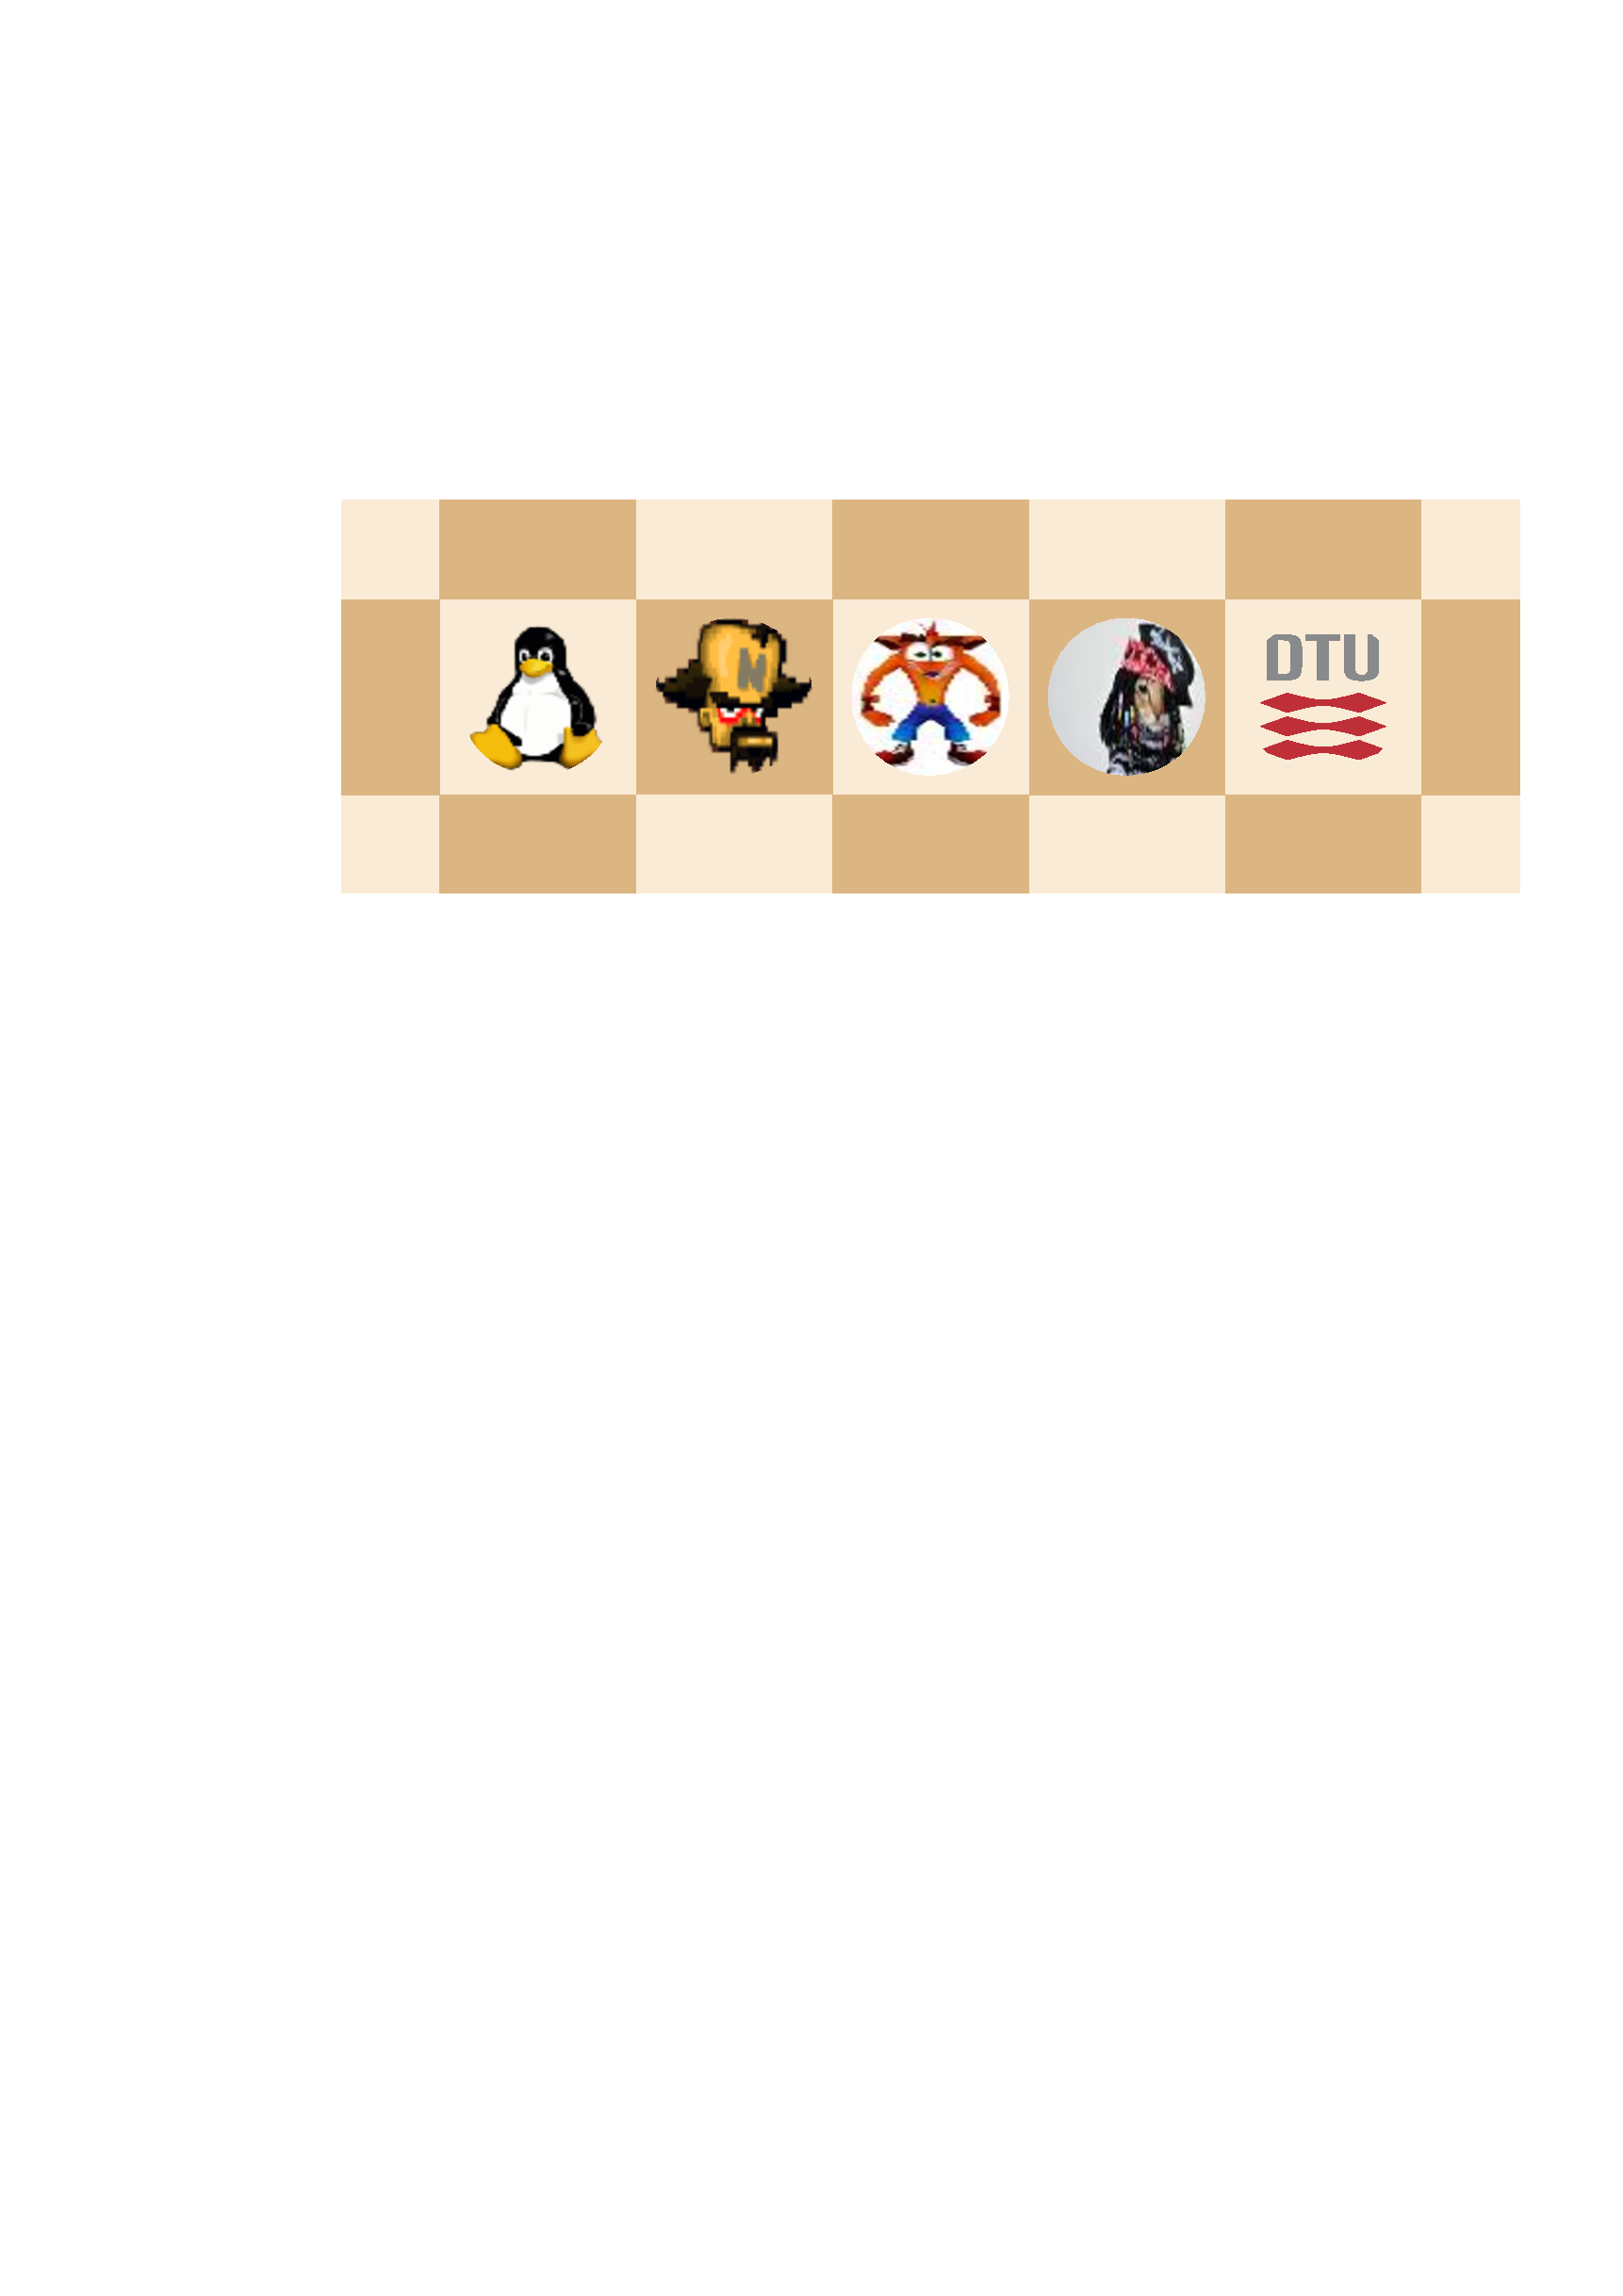
\includegraphics[width = 0.9 \textwidth]{Figurer/ShowcasePieces.pdf}
    \caption{Eksempler på billeder, spilleren kan uploade til sine brikker. Når spilleren vælger et billede, vil det bliver vist på alle spilleren brikker. Billedtyper understøttet: \texttt{.png, .jpeg, .gif, .jpg,  .bmp}.}
    \label{fig:ShowcasePieces}
    \end{figure}

%Jens
%Hvilke typer billeder kan jeg uploade? (gif, transparent)
\textbf{Tilpasselige brik-billeder:} Det er i spilindstillings menuen muligt at ændre på billederne brugt til begge holds brikker. Knapperne under \texttt{"Choose custom images"} åbner en \texttt{FileChooser} hvis tilladte extensions er: \texttt{ .png, .jpeg, .gif, .jpg,  .bmp}. Det valgte billede bliver gemt som et nyt objekt af typen \texttt{Image}. Herfra bliver billedet brugt til at danne et nyt objekt af typen \texttt{ImagePattern}. Dette format kan anvendes som et \texttt{Fill} i et \texttt{JavaFX Shape}. Det nye billede træder i kraft, når brugeren starter et nyt spil.\\

% Magnus
% Hvordan markeres kongebrikker? Billeder på billeder, eller udskift? (advdam)
\textbf{Kronet brik billede:} Hvis brugeren beholder standardbillederne på sine brikker, markeres kronede brikker yderligere ved udskiftning af billedet. Dette ses i figur \ref{fig:defaultPieces}. Den kronede brik har et guldbriller på! Dette er opnået ved at udskifte billedet på brikken, så hvis der uploades selvvalgte billeder, tilføjes der kun guldkant på brikken.  \\

\begin{figure}[H]
    \centering
    \includegraphics[width = 1.0\textwidth]{Figurer/DefaultPieces}
    \caption{Oversigt over standardbrikkerne for de to hold. Fra venstre til højre er det: Standard, valgt, kronet, kan dræbe og ikke valgbar.}
    \label{fig:defaultPieces}
    \end{figure}

%R  R
%   \item Hvad er gjort for at gøre spillet rart i gameplay? (advdam)
\textbf{Tilfredstillelse i spillet:} 
For at gøre spillet mere tilfredsstillende at spille er der tilføjet at brikker følger musen mens man flytter den, for at gøre hele oplevelsen mere virkelighedstro. Når man placerer en brik snapper den automatisk til feltets centrum.
\\

%   RR
%   \item Hvordan animeres spawn og død? 
\textbf{Animationer for spawn og død:} 
En brik spawnes ved at skaleres fra en prik med radius 0 til dens egentlige størrelse. Dette sker hver gang man går ind i spillet, uanset om det er et nyt spil eller et fortsat spil. En brik dræbes/fjernes ved at skaleres dem ned fra dens egentlige størrelse til en prik med radius 0. Dette sker hver gang en brik bliver dræbt. Målet med animationerne er at give en mere flydende overgang for spilleren. Pludselige ryk i brikker kan virke fejlfyldt og derfor uønsket.\\


% Magnus
% Hvad er begrænsningerne for spillet? (RAM) (advdam)
\textbf{Ressourcebegrænsninger for spillet:} Spillet virker ikke overvældende ressourcekrævende. Selv når spillet kører 50 gange 50 felter, og vi uploader gifs til brikkernes overflade, er det smooth. Ved 100 gange 100 felter med gifs er det ikke smooth, men spilbart. \\

%Jens
%Hvad gør continue knappen?
\textbf{Continue knappen:} Continue knappen skifter fra menuen tilbage til det spil der er i gang med at blive spillet.  \\

%   RR
%   \item Hvordan spiller jeg mod computeren?
\textbf{Spille mod AI:} 
Hvis man vil vælge at spille mod spillets AI gøres det gennem \texttt{"Settings"} menuen via checkboxen \texttt{"Play against computer"}.\\

%Jens
%Hvordan udløser jeg et uafgjort spil?
\textbf{Uafgjort spil:} Til højre i spil panelet findes to tie-checkboxes, én for hver spiller. Hvis begge er markeret afsluttes spillet og en besked i midten af brættet vises som fortæller at spillet er slut og endte uafgjort. \\
%   RR

%   \item Hvordan gemmer jeg og loader et spil?
\textbf{Loading af spil:}
Når spillet startes tjekkes om der findes en gyldig gemt fil. Hvis der findes en gyldig gemt fil vil \texttt{"Load"} knappen i main menu blive aktiv, hvis ikke vil den være inaktiv og først aktiveres igen når man gemmer spillet gennem \texttt{"Save"} knappen. Antaget at der findes en gyldig gemt fil og at man trykker på \texttt{"Load"} fra main menu, vil man blive dirigeret ind i spillet genereret fra den gemte fil. \\

% Magnus
% Er der lyde med? Hvorfor/hvorfor ikke?
\textbf{Lyde:} Vi eksperimenterede med lyde i tidligere versioner af programmet (baggrundsmusik, lyde ved drab), men det blev senere nedprioriteret. Vi har dog fået et indblik i, hvordan lyde kan tilknyttes events.